\documentclass[a4paper, twoside, 12pt]{report}
\usepackage[margin=2.5cm]{geometry}
\usepackage{fancyhdr}
\pagestyle{fancy}
\fancyhead{}
\fancyhead[RO,LE]{\small Macchine - ing. Meccanica - San Giovanni - Federico II - a.a. 2023/2024}
\renewcommand{\headrulewidth}{1pt}
\usepackage{amsfonts}
\usepackage{mathptmx}
\usepackage{amssymb}
\usepackage{microtype}
\usepackage{graphicx}
\usepackage{wrapfig}
\usepackage{enumitem}
\usepackage{index}
\usepackage{keyval}
\usepackage[italian]{babel}
\usepackage[font=small,labelfont=bf]{caption}
\usepackage{tikz, pgfplots}
\usepackage{subcaption}
\usepackage{amsmath}
\usepackage{cancel}
\usepackage{epigraph}
\usepackage{float}
\usepackage{ulem}

\begin{document}
	\title{\textbf{Esercizi di Macchine}}
	\author{di Salvatore Palumbo}
	\date{Anno accademico 2023-2024\\[10cm]
\includegraphics[width=14cm]{logo_uni.jpg}}
	\maketitle

\tableofcontents

\pagenumbering{arabic}
\setcounter{page}{2}
\chapter{Esercizio 1: Trasformazioni}
\section{Valutazione dello scambio di Energia meccanica e termica negli esempi proposti}
\paragraph{Compressione adiabatica isoentropica di 1 kg di aria da 1 bar e 288,15 K a 2,5 bar.\\}
In questo esempio si sta considerando una compressione adiabatica ($\delta q\;=\;0$) e isoentropica, quindi reversibile. L'equivalenza tra reversibile e isoentropica ci viene data dal bilancio di II legge: $TdS\;=\;\cancel{\delta q}\;+\;\delta q_{IRR}$ ($q$ si semplifica, essendo la trasformazione adiabatica). \\
Dalla termodinamica, sappiamo che ogni trasformazione reversibile può essere scritta attraverso un'unica trasformazione generica detta Politropica, definita a calore specifico costante:
\begin{center}
	$\delta q\;=\;c_{m}\;dT\;\implies\;pv^m\;=\;cost,\;\;\;m\;:=\; \frac{(c_{m}-c_{p})}{(	c_{m}-c_{v})}$
\end{center}
Compressione adiabatica $\implies\;\delta q\;=\;0\;\implies\;c_{m}\;=\;0\;\implies\;m\;=\;\frac{c_{p}}{c_{v}}\;=:\;k$
Quindi l'equazione che ottengo è: 
\begin{equation}
	pv^k\;=\;cost
\end{equation}
Questo prodotto è costante in ogni sezione del fluido, quindi posso scrivere che: $	pv^k\;=\;p_{1}v^k_{1}\;\implies$
\begin{equation}
	v\;=\;\Biggl(\dfrac{p_{1}v_{1}^{k}}{p}\Biggr)^\frac{1}{k}
\end{equation}
L'equazione dell'energia meccanica invece ci dice che per un sistema aperto:
\begin{equation}
	l_{12(SA)}\;=\;-\int_{1}^{2}vdp\;+\;\cancel{l_{attrito}}
\end{equation}
Sostituendo la (1.2) all'interno della (1.3), posso risolvere l'integrale ottenendo:
\begin{equation}
	H_{is}\;:=\;l_{12(SA)}\;=\;\dfrac{k}{k-1}\;R\;T_{1}\;\Biggl(1-\beta^\frac{k-1}{k}\Biggr)
\end{equation}
Quindi il lavoro meccanico che devo fornire dall'esterno per ottenere la compressione di questo gas(1 kg di aria $\implies k=1,4$) a queste condizioni di temperatura iniziale ($T_{1} = 288,15\; K$) per ottenere un rapporto di compressione ($\beta = \dfrac{p_{2}}{p_{1}} = \dfrac{2,5 bar}{1 bar} = 2,5$) è pari a:
\begin{center}
	$L_{12(SA)}\;=\;m\;l_{12(SA)}\;=\;1\;\cancel{kg}\;\dfrac{1,4}{1,4-1}\;287\;\dfrac{J}{\cancel{kg}\cancel{K}}\;288,15\;\cancel{K}\;\Biggl(1-2,5^\frac{1,4-1}{1,4}\Biggr)\;\approx\;-\;86621\;J\;\approx\;-\;86,6\;kJ$
\end{center}
Il segno negativo è atteso in quanto, per la convenzione scelta, lavori con segno positivo sono lavori in uscita dal sistema, mentre lavori con segno negativo entrano nel sistema. Nel caso di una compressione noi dobbiamo caricare il fluido, di un carico che nel caso adiabatico reversibile è proprio tutto il lavoro che abbiamo dato dall'esterno ($H_{is}=l_{12(SA)}$).\\
Come già detto essendo una compressione adiabatica reversibile non c'è nessuno scambio termico.
\begin{figure}[H]
	\centering
	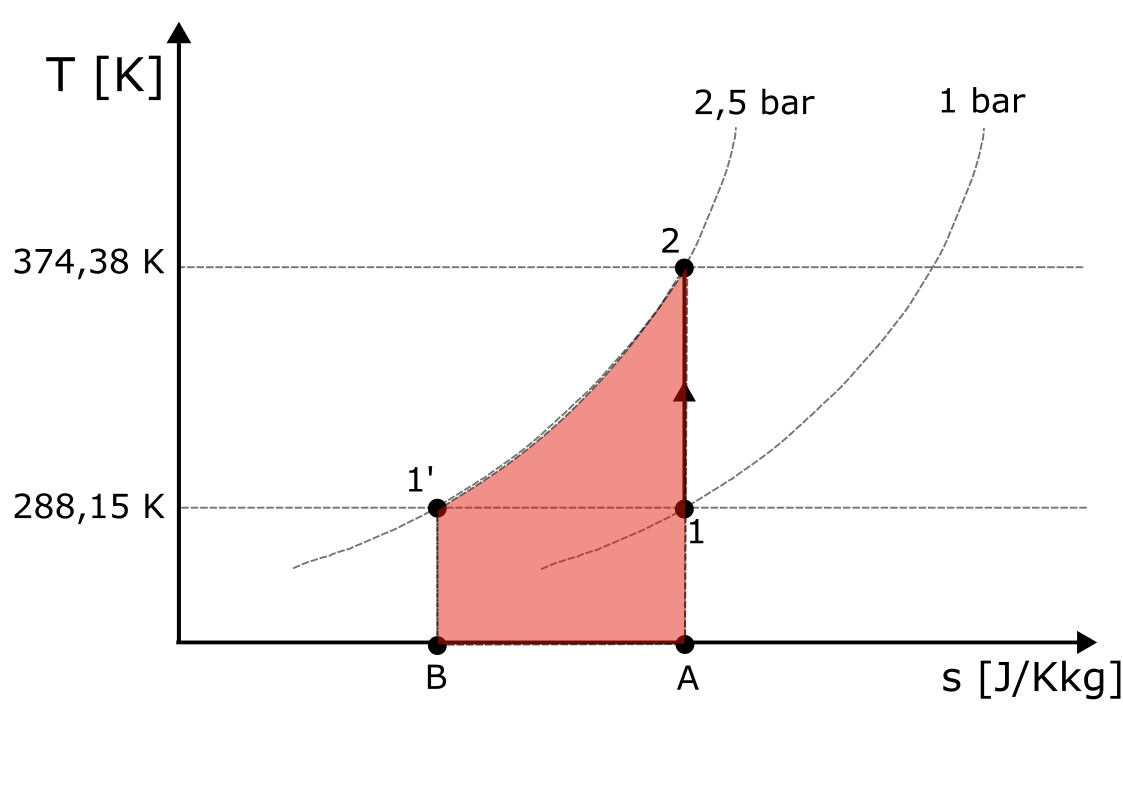
\includegraphics[width=0.9\textwidth]{adrev.png}
	\caption{Area B1'2A (in rosso) che rappresenta il lavoro}
\end{figure} 
Per visualizzare il lavoro sul piano T-s (piano del calore) si ricorre a un artificio. Consideriamo il punto 1' sull'isobara $p_{2}=2,5 bar$ che si trova alla stessa temperatura $T_{1}=288,15 K$ del punto 1.\\
Dato che per un gas l'entalpia dipende soltanto dalla temperatura $\implies\;h_{1}=h_{1'}$
\begin{center}
	$\implies h_{2}\;-\;h_{1}\;=\;h_{2}\;-\;h_{1'}\;=\;\int_{1'}^{2}dh\;=\;\int_{1'}^{2}Tds+v\cancel{dp}\;=\;Area(B1'2A)$
\end{center}
\newpage

\paragraph{Compressione adiabatica reale di 1 kg di aria da 1 bar e 288,15 K a 2,5 bar con $\eta_{pol}$ pari a 0,755.\\}
Durante una trasformazione reale, come quella di una compressione che avviene all'interno di un vero compressore, sono presenti delle irreversibilità interne dovute agli attriti. Pertanto, tale trasformazione non è una successione di infiniti stati di equilibrio e per questo motivo non è rappresentabile su un piano termodinamico. Per sopperire a questa mancanza, \uline{assumiamo che la compressione adiabatica reale ripercorra parimenti una compressione politropica reversibile con adduzione di calore}.\\ 
Tanto calore quanto è l'aliquota di lavoro, sottratta al totale fornito al sistema, che è stata degradata in calore dalle forze di attrito. Quindi per valutare lo scambio di energia necessario per ottenere questa compressione, si necessita di un parametro che ci dia informazioni sulla qualità della macchina. In questo esempio viene fornito il rendimento politropico:
\begin{equation}
	\eta_{pol}\;:=\dfrac{H_{pol}}{l_{r}}
\end{equation}
In maniera simile a quanto visto nella (1.3) e nella (1.4), il carico che conferisco al fluido è:
\begin{equation}
	H_{pol}\;=\;l_{12'}\;=\;-\int_{1}^{2'}v_{pol}dp\;=\;\dfrac{m}{m-1}\;R\;T_{1}\;\Biggl(1-\beta^\frac{m-1}{m}\Biggr)
\end{equation}
\uline{$H_{pol}\neq H_{is}$} perchè l'adduzione di calore che si ha nella politropica, fa si che ci sia un incremento della temperatura e di conseguenza un aumento del volume specifico $v_{pol}$. Il peggioramento delle condizioni di compressione è causa dell'ulteriore aliquota di lavoro che devo spendere per ottenere la stessa compressione del caso isoentropico:
\begin{center}
	$H_{pol}\;-\;H_{is}\;=\;controrecupero\;=\;Area(122')$
\end{center}
\begin{figure}[H]
	\centering
	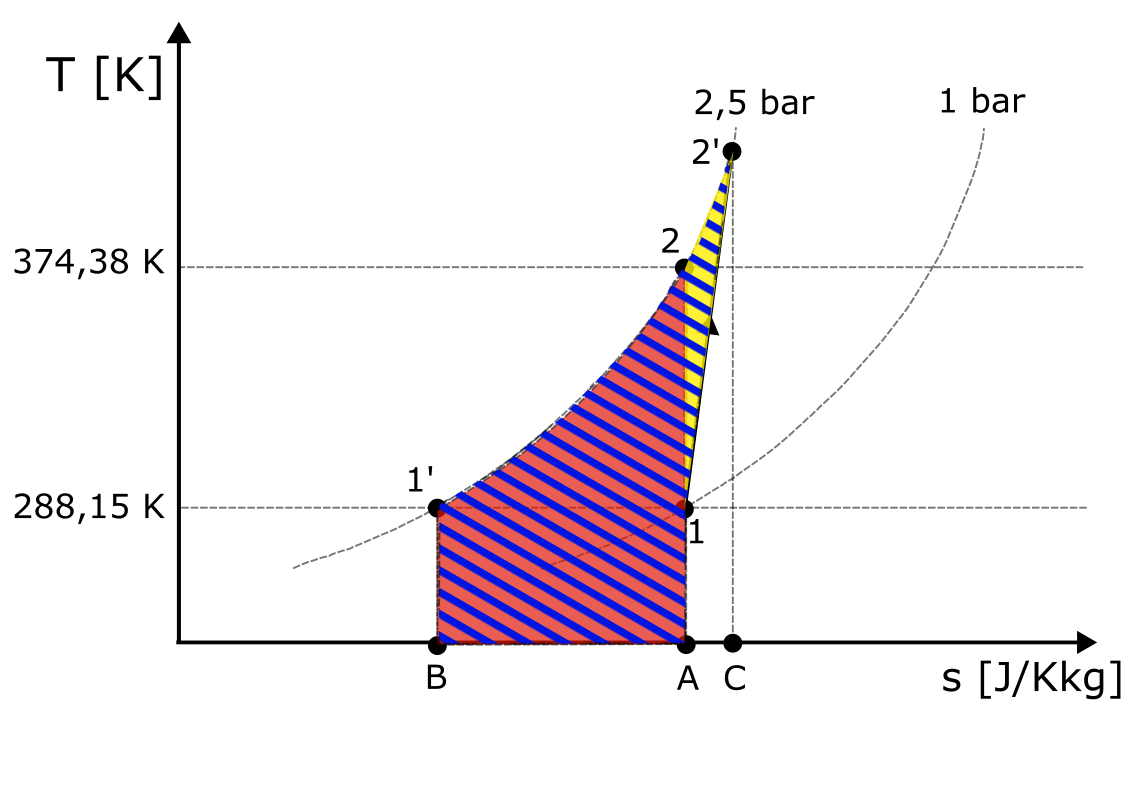
\includegraphics[width=0.9\textwidth]{caricopoliprotico.png}
	\caption{L' area B1'2A (in rosso) rappresenta il carico iso-s, l'area B1'2'1A(in blu) rappresenta il carico politropico mentre l'area 122' è il controrecupero}
\end{figure}
Il lavoro reale $l_{r}$ invece, in virtù della mia assunzione è il lavoro che mi permette di comprimere il gas ripercorrendo la stessa politropica ma senza addizionare ulteriore calore:
\begin{equation}
	l_{r}\;=\;-\int_{1}^{2'}v_{pol}dp\;+\;l_{attrito}\;=\;H_{pol}\;+\;l_{attrito}
\end{equation} 
Inoltre dal bilancio so che: 
\begin{equation}
	l_{r}\;=\;h_{1}\;-\;h_{2'}\;=\;c_{p}(T_{1}-T_{2'})=c_{p}\;T_{1}(1-\dfrac{T_{2'}}{T_{1}})=\;c_{p}\;T_{1}\;(1\;-\;\beta^{\frac{m-1}{m}})\;=\;\dfrac{k}{k-1}\;R\;T_{1}\;(1\;-\;\beta^{\frac{m-1}{m}})
\end{equation}
Quindi mettendo tutto assieme posso trovare una relazione che lega il rendimento politropico $\eta_{pol}$ con $k$ e $m$:
\begin{equation}
	\eta_{pol}\;=\dfrac{H_{pol}}{l_{r}}\;=\;\dfrac{\dfrac{m}{m-1}\;\cancel{R\;T_{1}\;\Biggl(1-\beta^\frac{m-1}{m}\Biggr)}}{\dfrac{k}{k-1}\;\cancel{R\;T_{1}\;\Biggl(1-\beta^\frac{m-1}{m}\Biggr)}}\;=\;\dfrac{\dfrac{m}{m-1}}{\dfrac{k}{k-1}}
\end{equation}
Quindi posso serenamente invertire e scrivere che: 
\begin{equation}
	m\;=\;\dfrac{\eta_{pol}}{\eta_{pol}-\frac{k-1}{k}}
\end{equation}
Quindi il coefficiente m è pari a:
\begin{center}
	contenuto...
\end{center}
\end{document}